% Working manuscript for Nature Sustainability (Article).
% main.tex is the editable manuscript. Migration is not run during compilation.
% Paragraph IDs preserve links to the dated Markdown evidence ledgers.
\documentclass[11pt,a4paper]{article}
\usepackage[T1]{fontenc}
\usepackage[utf8]{inputenc}
\usepackage{lmodern}
\usepackage[margin=25mm]{geometry}
\usepackage{amsmath}
\usepackage{graphicx}
\usepackage{microtype}
\usepackage[super,sort&compress,numbers]{natbib}
\usepackage[hidelinks]{hyperref}
\hypersetup{pdftitle={Evidence boundaries in AI-generated corporate sustainability disclosures},pdfauthor={}}
\graphicspath{{figures/}}
\setlength{\parindent}{0pt}
\setlength{\parskip}{0.5em}
\setlength{\emergencystretch}{2em}
\linespread{1.08}
\raggedbottom

\title{Evidence boundaries in AI-generated corporate sustainability disclosures}
\author{\normalsize AUTHOR\_INPUT\_NEEDED: authors and affiliations}
\date{\small Working draft --- 2 October 2026}

\begin{document}
\maketitle
\begin{center}
\small\textbf{Draft status.} Working title; Introduction, Results and Methods drafted.
Figures 1--4 are included; Abstract, Discussion and declarations remain incomplete.
\end{center}

\begin{abstract}
\textbf{DRAFT\_PENDING.} Write the abstract after the main argument and validation scope are settled.
The journal limit is 150 words, without references.
\end{abstract}

% Introduction has no printed section heading under the journal's Article structure.
% BEGIN_INTRODUCTION
% I01
Corporate sustainability reporting is intended to help users understand companies' material impacts on people and the environment, and how sustainability matters affect their business. The 2023 European Sustainability Reporting Standards (ESRS) articulate this purpose and require information to be complete, neutral and accurate. They describe verifiability as the possibility of corroborating information or the inputs used to derive it \cite{esrs2023}. These requirements make the connection between a disclosure and its evidence a central concern when reporting text is assembled from multiple company sources. A statement's usefulness depends partly on whether its meaning survives that transformation.

% I02
Large language models have been applied to sustainability-information analysis and disclosure drafting. ChatReport retrieves passages from corporate reports to answer questions and analyse climate-related disclosures \cite{chatreport2023}. SusGen-GPT uses retrieval-augmented generation (RAG) for sustainability report generation, incorporating information retrieved from annual reports into drafting prompts \cite{susgen2025}. Such workflows provide a concrete setting in which to examine the evidentiary basis of generated reporting statements. The availability of relevant source material does not, by itself, establish that a generated statement preserves the proposition supported by that material.

% I03
The difficulty extends beyond introducing facts absent from the source. A disclosure may retain familiar entities, actions or numbers while changing a qualification that determines their meaning. A description of a subsidiary's practice, for example, does not alone establish a group-wide practice, and evidence of an action in an earlier year does not necessarily establish its continuation in the reporting year. Similarly, an achieved outcome and a future target remain different propositions even when they concern the same metric. We use factual boundaries to denote such material qualifications, including entity, time, population, metric and certainty. Preserving them requires examining both individual facts and the relationships asserted when evidence is combined.

% I04
Existing evaluation methods provide foundations for this assessment. FActScore decomposes generated text into atomic facts and measures their support against a specified knowledge source \cite{factscore2023}; RAGAS and RAGChecker assess the support of response statements or claims in retrieved context \cite{ragas2024,ragchecker2024}. Context preservation and combined evidence are also established concerns. VeriScore retains necessary spatial and temporal modifiers in verifiable claims \cite{veriscore2024}, while Claimify uses context to resolve ambiguity during claim extraction \cite{claimify2025}. ALCE evaluates whether concatenated cited passages support a statement \cite{alce2023}. These approaches motivate explicit treatment of claim meaning and evidentiary scope when adapting support assessment to sustainability reporting.

% I05
Sustainability-specific work provides direct precedents as well. ChatReport evaluates answer support and source attribution with human annotators and documents an erroneous concatenation of separate retrieved chunks \cite{chatreport2023}. ESG-Bench provides human annotations of support and hallucination in ESG question answering \cite{esgbench2026}. Building on this work, the measurement question for disclosure drafting is how to characterize support while preserving material reporting qualifiers and distinguishing warranted inference from unsupported synthesis. An explicit account of the evidence considered, the proposition assessed and the reason for an unsupported judgment can make disagreements open to inspection.

% I06
Here we develop and apply Boundary-Aware Claim Evaluation (BACE) to investigate the extent, forms and assessment of evidentiary support in AI-generated sustainability disclosures. BACE links claims extracted from disclosures to candidate claims extracted from the evidence supplied to the generator, distinguishes direct from inferred support, and assigns reporting-oriented diagnoses to unsupported claims. We analyse 1,798 completed disclosures from a planned design of 1,800 company--year--task cases spanning 30 companies, reporting years 2019--2023 and 12 tasks based on the 2023 ESRS edition. We describe support patterns and automated diagnoses, inspect source-linked cases, and compare assessments with the native faithfulness scores of RAGChecker and RAGAS. The analysis concerns one fixed retrieval and generation workflow. Its judgments are conditional on claim extraction and candidate evidence selection; they measure supplied-evidence support, not external truth or legal compliance. The contribution is a reporting-focused operationalization and empirical comparison whose automated judgments remain subject to independent validation.
% END_INTRODUCTION

% BEGIN_RESULTS
\section*{Results}

\subsection*{Study scope and boundary-aware evaluation}

% R01
We examined the evidentiary support of corporate sustainability disclosures generated for 30 companies across five reporting years, 2019--2023, and 12 tasks based on the 2023 European Sustainability Reporting Standards (ESRS). The tasks covered climate change, own workforce and business conduct. The design specified 1,800 company--year--task cases; 1,798 had completed BACE assessments and available scores from both comparison methods and formed the analysed cohort (Fig.~\ref{fig:1}). The two incomplete BACE cases were excluded from support summaries and paired comparisons. Each disclosure was generated using a fixed retrieval and generation configuration, with narrative passages, table rows and structured metrics drawn from the permitted company-specific source years.

% R02
Boundary-Aware Claim Evaluation (BACE) reconstructed support relationships between claims extracted from each generated disclosure and claims extracted from its supplied evidence. A disclosure claim received direct support when an accepted evidence set explicitly entailed its complete meaning, and inferred support when entailment required a necessary reasoning step. Claims with no accepted support set were classified as unsupported. Material qualifiers, including entity, period, population, metric and certainty, formed part of the proposition being assessed. These judgments operated on extracted claims and selected candidate evidence claims (Fig.~\ref{fig:1}); they assessed support within the supplied evidence boundary rather than independently verified corporate facts.

\subsection*{Evidentiary support across disclosure tasks}

% R03
Across the 1,798 completed disclosures, the mean disclosure-level BACE support rate was 55.4\% (95\% company-cluster bootstrap interval, 53.9--56.8\%; Fig.~\ref{fig:2}a). This estimate gave each disclosure equal weight and counted both direct and inferred support. Pooling claims instead yielded a support rate of 55.1\%: of 94,955 deduplicated disclosure claims, 34,430 received direct support (36.3\%), 17,879 received inferred support (18.8\%) and 42,646 were classified as unsupported (44.9\%; Fig.~\ref{fig:2}b). The pooled proportions describe claims, whereas the disclosure-level mean describes the average assessed disclosure.

% R04
Mean support varied across the reporting tasks, from 43.9\% for workforce targets (S1-5) to 62.5\% for business conduct policies (G1-1; Fig.~\ref{fig:2}c). The workforce-policies and workforce-targets tasks each contributed 149 completed disclosures; the other tasks each contributed 150. These differences describe the observed workflow and evidence configuration. They do not isolate task difficulty or establish that one reporting topic is intrinsically more amenable to evidence-supported generation.

% R05
The primary support denominator retained all extracted disclosure claims, including assertions that information had not been disclosed or supplied. Excluding claims assigned the non-disclosure-statement diagnosis increased the support rate by a median of 1.9 percentage points within disclosures, with a maximum change of 58.0 percentage points. This sensitivity analysis shows that such assertions materially affect some disclosure-level scores. Neither denominator converts an automated unsupported proportion into a factual-error rate.

\subsection*{Patterns of unsupported disclosure claims}

% R06
Factual boundary distortion and evidence conflation together accounted for 31,335 of the 42,646 unsupported-claim diagnoses (73.5\%; Fig.~\ref{fig:3}a). BACE assigned factual boundary distortion to 19,130 claims (44.9\% of unsupported claims) and evidence conflation to 12,205 (28.6\%). The remaining diagnoses were non-disclosure statements, inferential inflation, unsupported novelty and contradiction. Boundary distortion denotes a transfer of an anchored fact beyond a material qualifier; conflation denotes an unsupported relationship constructed from separately evidenced elements. These are mutually exclusive outputs of an ordered diagnostic procedure, rather than independently established frequencies of underlying reporting errors.

% R07
A temporal example illustrates why the reporting context matters to those judgments (Fig.~\ref{fig:3}b). In a disclosure generated for Wärtsilä's 2022 supplier-relationships task, the statement that the company uses an online solution for supply-chain risk identification was assigned factual boundary distortion. The cited evidence explicitly describes such a solution in a 2019 report. BACE disputed whether that historical description established use in the target reporting context; the source does not establish that the company subsequently discontinued the solution. This ambiguity is relevant to the study design, in which PDF evidence precedes the target reporting year, while structured metrics may include that year.

% R08
Source inspection also exposed a limitation in an automated diagnosis (Fig.~\ref{fig:3}c). For ASML's 2019 emissions disclosure, a contradiction rationale relied on an extracted evidence claim that associated electricity-consumption conversion factors with direct Scope 1 emissions. In the original 2018 report glossary, those factors belong to the adjacent indirect Scope 2 entry; the direct Scope 1 entry instead refers to natural-gas combustion and purchased carbon dioxide. Flattening the glossary had obscured the row association. This case challenges the recorded contradiction rationale and demonstrates why diagnostic counts must be interpreted alongside the transformations from source documents to evidence claims.

\subsection*{Differences among automated evaluators}

% R09
The same 1,798 disclosures received mean native faithfulness scores of 90.2\% from RAGChecker and 90.7\% from RAGAS, compared with BACE's mean support rate of 55.4\% (Fig.~\ref{fig:4}a). Mean within-disclosure differences, calculated as BACE minus comparator, were \ensuremath{-}34.9 percentage points for RAGChecker (95\% company-cluster bootstrap interval, \ensuremath{-}36.2 to \ensuremath{-}33.5) and \ensuremath{-}35.3 percentage points for RAGAS (\ensuremath{-}36.5 to \ensuremath{-}34.1; Fig.~\ref{fig:4}b). These comparisons paired disclosures but retained each method's native claim inventory and scoring procedure.

% R10
The median numbers of claims per disclosure were 52 for BACE, 40 for RAGChecker and 42 for RAGAS (Fig.~\ref{fig:4}c). Thus, matching the generated text and supplied evidence did not produce identical sets of evaluated propositions. The internal checking contexts also differed: RAGChecker checked individual evidence cards, RAGAS used their combined context, and BACE assessed selected extracted evidence claims (Methods). Inventory size alone does not explain the score differences, and the differences do not establish an accuracy ranking. We therefore inspected specific native judgments against the generated passages and their complete supplied evidence.

% R11
One disagreement changed the unit being counted. In SCA's generated 2022 corruption-and-bribery disclosure, five incidents involving worker dismissal or discipline became five workers dismissed or disciplined. The supplied indicator counted incidents, without specifying the number of distinct workers. BACE classified the claim as unsupported and diagnosed factual boundary distortion. Both RAGChecker and RAGAS retained the five-worker proposition in their extracted claims and marked it supported. RAGAS's justification itself referred to five incidents. Because an incident count does not determine a distinct-worker count, the shared positive judgments accepted a proposition that the supplied indicator did not establish.

% R12
A population distinction appeared in Continental's generated 2021 workforce disclosure. One supplied indicator reported 62\% employee coverage by qualifying health and safety management systems; another reported 62\% audited or certified system coverage for own workers. The generated passage combined these into an employee-specific audited-coverage percentage. Both comparators accepted that proposition, whereas BACE diagnosed evidence conflation. The supplied records contained no definition equating the two populations for this indicator. Identical percentages did not establish the employee-specific audited-coverage rate, although they also did not prove that the company's actual rate differed.

% R13
A climate-related disagreement concerned the role assigned to an emissions value. Banco BPM's generated 2023 disclosure described a strategic plan envisaging a reduction from 17.5 thousand to 7.4 thousand tonnes of carbon dioxide equivalent. Both comparators accepted the planned-reduction interpretation; RAGChecker explicitly labelled 7.4 thousand tonnes as the target. The supplied table row contained both numbers but had lost their column headings. Inspection of the original 2022 report showed that 17.5 thousand tonnes was the 2019 value, 7.4 thousand tonnes was the 2022 status, and the target column specified carbon neutrality during the plan horizon. BACE returned unsupported, but its candidate evidence claims omitted the numerical cells. Its verdict therefore does not demonstrate recovery of the original table structure.

% R14
These targeted cases locate disagreements in counting units, population qualifiers and the attribution of values to outcomes or targets. They complement the aggregate comparison by showing which propositions were accepted, while the source-extraction counterexample identifies a limitation within BACE. The cases were selected through lexical screening followed by inspection of complete passages and supplied evidence (Methods). They do not provide representative error frequencies or independent human validation of any evaluator.
% END_RESULTS

\section*{Discussion}
\textbf{DRAFT\_PENDING.} Interpret the results in relation to disclosure evidence credibility,
the literature and the study's measurement boundaries. Preserve the source-extraction
counterexample, native-comparator limitations and the actual human-assessment status.

% BEGIN_METHODS
\section*{Methods}

\subsection*{Study design and company selection}

% M01
We evaluated one fixed retrieval and generation workflow for corporate sustainability disclosure. The observational unit was a generated disclosure for one company, target reporting year and task. The source register contained 600 companies; 250 met the source-availability criteria. Eligibility required a known latest primary Sustainable Industry Classification System sector at or before 2023, at least one extracted structured-metric record marked valid and containing a nonempty value in every source year from 2015 to 2023, and a locally available PDF with a valid file header in every source year from 2015 to 2022. Subsequent parsing checked annual narrative availability. Eligibility did not depend on task-specific metrics or evaluator scores, but restricted the study to companies with the required source coverage. The manuscript questions and descriptive comparisons were organized after the experiment and were not preregistered hypotheses.

% M02
We selected 30 companies across the 11 eligible sectors. One place was allocated to each sector; the remaining 19 were allocated by Hamilton largest remainders, weighted by eligible sector size minus one, with alphabetical tie-breaking. Within each sector, company identifiers were sorted and shuffled using Python's pseudorandom generator, initialized with the integer SHA-256 digest of the string comprising the sampling seed, 20260916, a colon and the sector name. The first companies up to the sector quota were selected, with the remainder forming an ordered reserve. The protocol permitted replacement by the next same-sector reserve if a required source year proved unusable before generation, but prohibited replacement on generated content or evaluation results. No replacement was recorded for this draw.

\subsection*{Disclosure tasks and temporal evidence boundaries}

% M03
Each company was assigned 12 tasks in each target reporting year from 2019 to 2023, giving a planned matrix of 1,800 cases. Task definitions used the 2023 European Sustainability Reporting Standards as a common framework: climate transition plans, actions and resources, targets, and greenhouse gas emissions (E1-1, E1-3, E1-4 and E1-6); workforce policies, actions and resources, targets, and health and safety metrics (S1-1, S1-4, S1-5 and S1-14); and business conduct policies, supplier relationships, anti-corruption controls, and corruption and bribery incidents (G1-1 to G1-4). Applying these definitions to earlier reporting years specified a generation task; it did not establish a legal obligation for each company and year.

% M04
For target year \(t\), structured metrics were eligible from source years \(t-4\) through \(t\), whereas PDF reports were eligible from \(t-4\) through \(t-1\). These were report-year filters, not publication-date cutoffs. Reports could describe measurements from other periods or prospective commitments, whose temporal qualifiers remained relevant to support. The historical PDF window could therefore limit evidence for claims about current practices, even where current-year structured metrics were available. Disclosures generated for other tasks were not supplied as evidence.

\subsection*{Evidence preparation and retrieval}

% M05
The evidence corpus combined structured-metric cards rendered deterministically from an existing extraction CSV, narrative passages extracted from reports with PyMuPDF, and table rows extracted with pdfplumber. Narrative preparation used the recorded 40--250-word chunking rules. Eligible reports were processed without task-keyword page selection. Stable evidence identifiers, source years, file hashes and source references were retained; PDF cards also retained page locations. Structured-metric cards represented extracted CSV records and were not treated as independently verified quotations from original reports. Flattening narrative and table layouts could alter relationships between labels and values.

% M06
Before generation, a quality gate excluded an entire card if it contained at least ten unmapped private-use or replacement glyphs comprising more than 5\% of non-whitespace characters, or exceeded 8,191 tokens under the cl100k\_base tokenizer. The preparation record also identifies four quarantined Evonik 2023 metric mappings following source inspection. Original reports and exclusion records were retained, and source-year availability was rechecked after quarantine. These checks addressed specified extraction problems without certifying the remaining source representations. Missing metrics and evidence types were not imputed.

% M07
Retrieval combined BM25 with cosine similarity over 3,072-dimensional text-embedding-3-large embeddings. Company and source-year filters were applied before ranking. Each channel retrieved up to 200 candidates per task subquery; reciprocal rank fusion combined subquery rankings within channels and then the channel rankings, using a rank constant of 60. Stored corpus vectors were already normalized; the retrieval configuration disabled additional corpus normalization. Ties were resolved by best individual rank, most recent source year and evidence identifier. The final selection retained up to ten cards from each evidence type, without a reranker or redistribution of unfilled quotas. Evidence entered the generation prompt in narrative, table-row and structured-metric order. Thus, 30 cards was a maximum, not a requirement for every case. The query bundles, selected card order and generation inputs were saved before the main run.

\subsection*{Disclosure generation and incomplete cases}

% M08
Generation used the configured Azure OpenAI gpt-5.6-sol deployment, with recorded model-version label 2026-07-09, medium reasoning effort, no temperature parameter and an output budget of 8,192 tokens. The shared prompt requested a professional disclosure of 300--500 words based on the supplied evidence. The first complete response meeting the length rule was accepted. Incomplete or out-of-range responses triggered up to two retries of the identical prompt per invocation, with rejected attempts retained; response selection did not use evaluator scores. The runtime permitted at most three attempts per stage. These settings and saved outputs document the executed workflow but do not guarantee byte-identical responses from a later remote deployment.

% M09
Generation preceded the BACE, RAGChecker and RAGAS evaluation branches. Stage receipts recorded dependencies and artifact hashes so that verified completed work could be reused after interruption. Unresolved evaluations remained missing. The saved analysis contained 1,798 completed BACE cases, all with available native comparator scores. Banco BPM's 2019 workforce-targets case and Investec's 2023 workforce-policies case had incomplete BACE branches and were excluded without zero imputation. Their exclusion did not imply failure of generation or of every comparator branch. The analysed cohort and saved run status were retained explicitly rather than treating the planned matrix as fully completed.

\subsection*{BACE claim construction and support judgments}

% M10
BACE first constructed evidence claims (ECs) from the complete prompt-visible evidence and disclosure claims (DCs) from the generated disclosure. The fixed sequence comprised direct extraction version 8, identified-patch review version 4 using operational definition version 2, constrained atomicity review version 2, and semantic deduplication within each case. The BACE stage configurations selected Azure gpt-5.6-sol, with model-version label 2026-07-09 and medium reasoning effort. The extraction rules required material qualifiers, including entity, period, population, metric, unit and certainty, to remain attached to their propositions. Each initial EC was attributed to one evidence card, and deduplication retained source-occurrence lineage. The configured schema-only acceptance mode did not require a quoted string to match its source exactly; stored quotation fields consequently did not establish verified attribution.

% M11
Candidate selection operated on the deduplicated EC and DC texts. It did not receive retrieval scores, task definitions or separate source-provenance fields as additional factual premises. For each DC, the support judge received the DC text, selected candidate EC identifiers and texts, company name and target reporting year. It did not receive the original evidence cards or the full unselected EC inventory at this stage. Company and year provided interpretive context but could not supply absent facts. Support decisions were therefore conditional on the preceding extraction and candidate selection.

% M12
The support prompt requested every distinct minimal sufficient EC set that supported the complete DC, including its material qualifiers. Minimality meant that removing any member would leave that set insufficient; it did not require choosing only the smallest set among all alternatives. A set was direct when it explicitly entailed the claim, allowing equivalent wording, and inferred when entailment required a necessary reasoning step rather than a merely plausible assumption. Support type did not depend on the number of ECs in a set. Any accepted direct set produced a direct DC verdict; accepted inferred sets without a direct set produced an inferred verdict; no accepted set produced an unsupported verdict. An empty candidate set yielded an empty support result without a support-model call. The output contained support sets and their types, rather than a prose support rationale. Structural validation checked identifiers and record completeness, but did not independently establish the semantic validity, minimality or exhaustiveness of the returned sets.

% M13
Each unsupported DC received one diagnosis, assigned in a fixed precedence order. A non-disclosure statement asserted an absence of disclosure or evidence within a specified scope. Contradiction required an incompatible proposition at matching material boundaries. Evidence conflation combined elements from multiple ECs into an unsupported relationship or attribution. Factual boundary distortion transferred an anchored fact across a material qualifier, such as entity, time, population, metric or unit. Inferential inflation strengthened meaning, status, certainty or conclusion beyond the evidence while retaining the relevant factual boundaries. Unsupported novelty applied when no candidate EC anchored the core proposition. These mutually exclusive outputs characterized the automated diagnostic procedure. Assertions about absent information entered support assessment first and were not automatically assigned an unsupported diagnosis.

\subsection*{Outcomes and native comparator procedures}

% M14
For disclosure \(d\), let \(N_d\) be the number of deduplicated DCs, and \(A_d\) and \(I_d\) the numbers receiving direct and inferred support. The primary support rate was

\[
s_d=\frac{A_d+I_d}{N_d}.
\]

The disclosure-level mean gave each completed disclosure equal weight, whereas the pooled estimate divided total supported claims by total DCs:

\[
\bar{s}=\frac{1}{n}\sum_{d=1}^{n}s_d,
\qquad
s_{\mathrm{pooled}}=\frac{\sum_d(A_d+I_d)}{\sum_d N_d}.
\]

Diagnosis proportions used all unsupported DCs as their denominator. The metric implementation required nonempty EC and DC inventories, complete support records and diagnoses that exactly partitioned unsupported DCs; invalid or incomplete cases did not receive fabricated scores.

% M15
For sensitivity analysis, \(Z_d\) denoted the number of unsupported DCs diagnosed as non-disclosure statements. The alternative rate was \((A_d+I_d)/(N_d-Z_d)\), and its change from \(s_d\) was summarized within disclosures in percentage points. This removed only claims assigned that diagnosis. Additional saved metrics were evidence-claim coverage, defined as the number of distinct ECs appearing in any accepted support set divided by the total deduplicated EC inventory, and inference rate, defined as \(I_d/(A_d+I_d)\). Zero denominators produced missing values. Inference rate differed from the inferred share of all DCs reported in Results; coverage described use of supplied extracted evidence, not completeness of corporate reporting.

% M16
RAGChecker evaluates claim-level entailment and defines faithfulness through support in retrieved context \cite{ragchecker2024}. RAGAS assesses faithfulness by extracting response statements and checking their support in the supplied context \cite{ragas2024}. We used RAGChecker 0.1.9 with RefChecker 0.2.13 and RAGAS 0.4.3. A common adapter supplied the same generated response and ordered prompt-visible evidence, checking prompt, response and context hashes. Each comparator retained its native extraction prompts, checking procedure and claim denominator. Only faithfulness was evaluated; no reference answers were supplied. The configured Azure gpt-5.6-sol judge used medium reasoning. The transport adapter supplied these reasoning and output-budget settings in place of package-default request parameters while preserving native prompts and scoring.

% M17
In the recorded RAGChecker procedure, extracted response triplets were checked against individual evidence cards; a claim counted as supported if at least one card received an entailment verdict. The joint-checking group size was five claims, not five merged evidence cards. RAGAS checked its extracted statements against the combined supplied contexts and calculated their supported fraction. Invalid extraction, response or statement-alignment outputs were subject to the recorded retry policy and remained missing if unresolved. Matching source inputs at the adapter level did not align the evaluated propositions or make either comparator's checking context identical to BACE's candidate ECs. Native score differences could therefore reflect multiple stages and did not isolate evaluator accuracy.

\subsection*{Aggregation and uncertainty}

% M18
We reported disclosure-level and task-level means, pooled claim counts and diagnosis composition using the completed cohort. Paired comparisons used the intersection of available BACE, RAGChecker and RAGAS scores. For each comparator, its score was subtracted from BACE's support rate within each disclosure before averaging; differences were expressed in percentage points. Native claim-count medians used the same paired disclosures. No sector population weights were applied, and claims from different native inventories were not treated as matched measurement units.

% M19
The saved analysis used 2,000 company-cluster bootstrap draws with NumPy's default random generator and seed 20260921. Each draw sampled companies with replacement and retained every observed disclosure from each sampled company, including multiplicities. For each mean or paired difference, the statistic divided the sum of the resampled disclosure values by their resampled count. Thus, clustering accommodated repeated years and tasks within companies while preserving disclosure weighting. The 2.5th and 97.5th percentiles formed the reported 95\% intervals. Task-specific calculations used the observed disclosures for that task. The analysis was descriptive and did not perform significance tests. These intervals did not include uncertainty from additional model runs, extraction, human annotation or unresolved cases, and did not implement a sector-design-adjusted extrapolation to the register.

\subsection*{Selection and source inspection of illustrative cases}

% M20
The fixed diagnostic illustrations originated in within-label candidate pools that required a localizable quotation in the generated text. The Wärtsilä temporal case and ASML contradiction case used the recorded selection seeds 20260924 and 20260922, respectively. These case identifiers were retained during manuscript preparation. Source inspection assessed whether their particular rationales preserved the evidence's temporal or tabular relationships; it did not validate the complete disclosures. The ASML example was retained because the original glossary challenged the recorded contradiction rationale.

% M21
Additional comparator disagreements were discovered through targeted screening of saved outputs. The initial screen considered BACE contradictions and other unsupported DCs with an exact normalized match to a supported RAGAS statement. It then identified the nearest native claims by token-set Jaccard overlap and retained candidates with positive judgments from both comparators. A supplementary screen searched unsupported quantitative DCs containing a digit and a specified unit or status keyword, excluded non-disclosure statements, and required both nearest native claims to be supported with Jaccard overlap of at least 0.65. Exact normalization used Unicode NFKC, case folding and word-token joining. These lexical operations retrieved candidates; they did not establish semantic equivalence or representative error frequencies.

% M22
For the selected SCA, Continental and Banco BPM cases, inspection compared the complete generated passage, all supplied evidence cards, the disputed DC, its candidate ECs and the exact native statements and verdicts. Candidates were not promoted as clear shared disagreements when a native statement omitted the disputed qualifier, another supplied card established support, or the complete passage qualified the apparent overstatement. The original Banco BPM report was inspected after evaluation to resolve column headings missing from the supplied table row; those restored headings were not evaluator inputs. Its BACE candidate ECs omitted the numerical cells, so an unsupported verdict did not demonstrate recovery of the original structure. These source-linked inspections were part of manuscript preparation, with AI assistance, and were not independent human annotation or estimates of evaluator accuracy.

\subsection*{Prepared independent human assessment}

% M23
An independent assessment package was prepared to examine BACE judgments conditional on their actual DC and candidate EC inputs. The formal design documented on 25 September 2026 replaced the broader source-review scope described in the original protocol. It selected 600 unique DCs from the completed inventory: 400 primary units, allocated proportionally across automated direct, inferred and unsupported strata using largest remainders, and 200 supplementary units from the remaining unsupported pool. Primary quotas were 145, 75 and 180, respectively. Selection used seeded SHA-256 ranking without replacement, with seed bace-human-validation-v1-20260924. Supplementary allocation successively favoured the least represented diagnosis, breaking ties in the fixed diagnostic order and capping total contradiction units at 40 to retain calibration-eligible units. An independent seeded ranking set the presentation order, with group membership withheld from reviewer workbooks.

% M24
Two workbooks contained the same 600 sample identifiers and supplied company name, target year, complete DC text and the exact candidate EC membership, order, identifiers and wording. Automated answers were omitted, and the instructions required independent review without access to the other reviewer's answers. As of the local file check on 1 October 2026, both workbooks had blank support and diagnosis cells; the manifest recorded prepared, not annotated, and calibration had not been conducted. No reviewer agreement, adjudication or accuracy estimates were available from these files. This status describes the inspected local copies and does not establish whether completed annotations exist elsewhere.

% M25
The prepared design specifies primary-stratum weights for overall estimates from the 400 primary units. Supplementary inclusion probabilities are conditional on the realized primary sample; the combined 600 units must not be analysed as an unweighted representative sample. Reviewers are to assign direct, inferred or unsupported labels and one diagnosis only when selecting unsupported. Any future calibration must use separate units. The supplied material permits assessment of conditional support and diagnosis decisions, but not independent validation of extraction, candidate selection, original-source completeness, real-world truth or comparative evaluator accuracy. Reviewer qualifications, completed calibration, agreement procedures and adjudication outcomes require documentation before reporting human-assessment results.
% END_METHODS

\section*{Data availability}
\textbf{AUTHOR\_INPUT\_NEEDED.} Verify the repository, release identifier and access
conditions for the minimum supporting dataset, including third-party input restrictions.

\section*{Code availability}
\textbf{AUTHOR\_INPUT\_NEEDED.} Verify the code release, persistent identifier and
review-access route before making a deposit or availability claim.

\bibliographystyle{unsrtnat}
\bibliography{references}

\section*{Acknowledgements}
\textbf{AUTHOR\_INPUT\_NEEDED.} Confirm acknowledgements and funding information.

\section*{Author contributions}
\textbf{AUTHOR\_INPUT\_NEEDED.} Confirm the author list and actual contributions.

\section*{Competing interests}
\textbf{AUTHOR\_INPUT\_NEEDED.} Obtain and record the authors' declarations.

\section*{AI-use statement (draft)}
AI assistance was used in manuscript drafting and formatting.\par
\textbf{AUTHOR\_INPUT\_NEEDED.} Specify the tools and the authors' completed oversight
and verification, and integrate the disclosure in the appropriate manuscript location.

\clearpage
\section*{Figures}

\begin{figure}[!htbp]
\centering
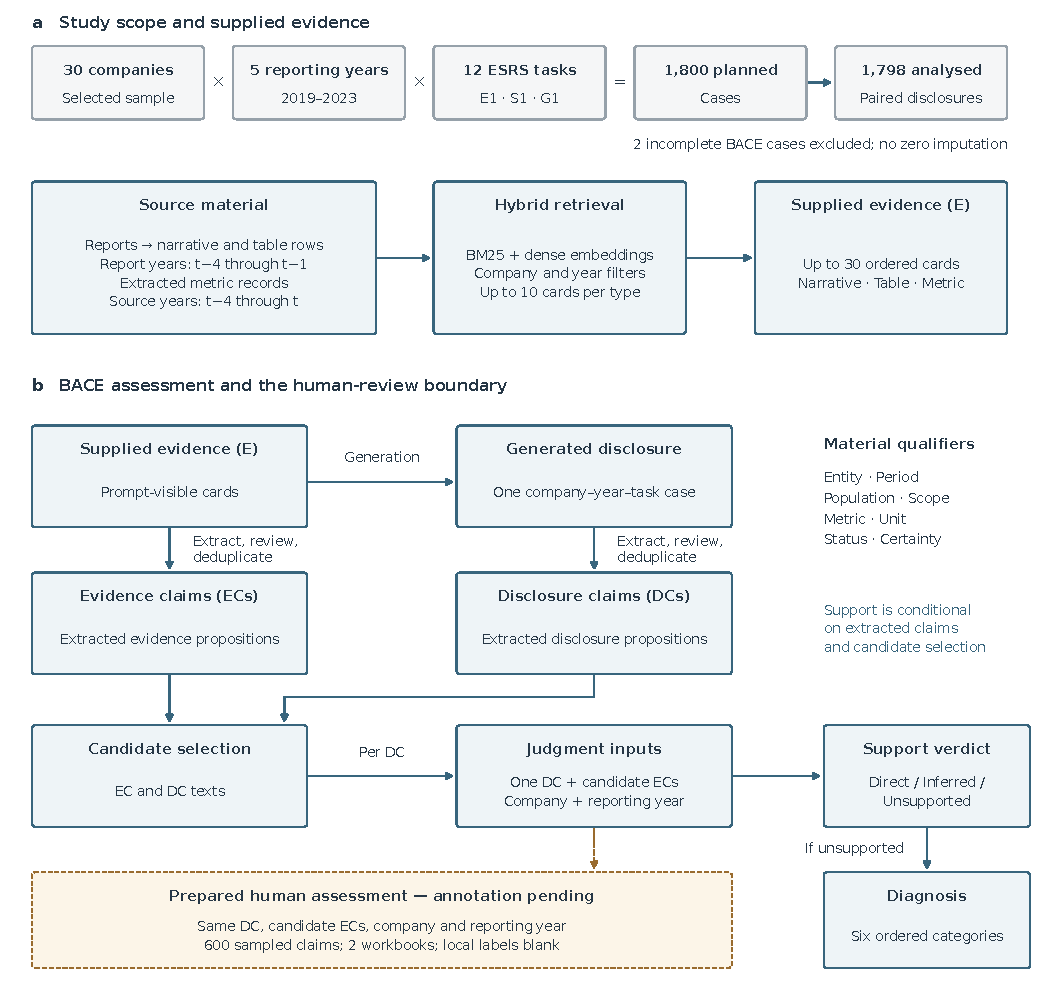
\includegraphics[width=\linewidth]{fig1_study_design.pdf}
\caption{\textbf{Study design and evidence boundaries.}
\textbf{a,} The planned matrix comprises 30 companies, five reporting years (2019--2023) and 12 disclosure tasks.
Of 1,800 planned cases, 1,798 have completed BACE assessments and both native comparator scores;
two incomplete BACE cases are excluded without zero imputation.
For target reporting year \(t\), PDF reports supply narrative and table evidence from \(t-4\) through \(t-1\),
while extracted metric records cover \(t-4\) through \(t\).
These are source-year filters, not publication-date cutoffs.
Retrieval supplies up to ten cards per evidence type, with a maximum of 30.
\textbf{b,} Solid arrows trace automated processing.
Evidence claims (ECs) and disclosure claims (DCs) are constructed by extraction, review and deduplication.
Candidate selection uses EC and DC texts.
Support assessment receives one DC, its selected candidate ECs, company and reporting year,
and assigns direct, inferred or unsupported verdicts.
Only unsupported DCs receive one of six ordered diagnoses.
The dashed amber branch marks prepared human assessment using the same judgment inputs:
two reviewer workbooks contain the same 600 sampled DCs, with annotation cells blank in the inspected local copies.
Support judgments remain conditional on extraction and candidate selection;
neither those judgments nor the prepared review establishes external corporate truth.}
\label{fig:1}
\end{figure}

\clearpage
\begin{figure}[!htbp]
\centering
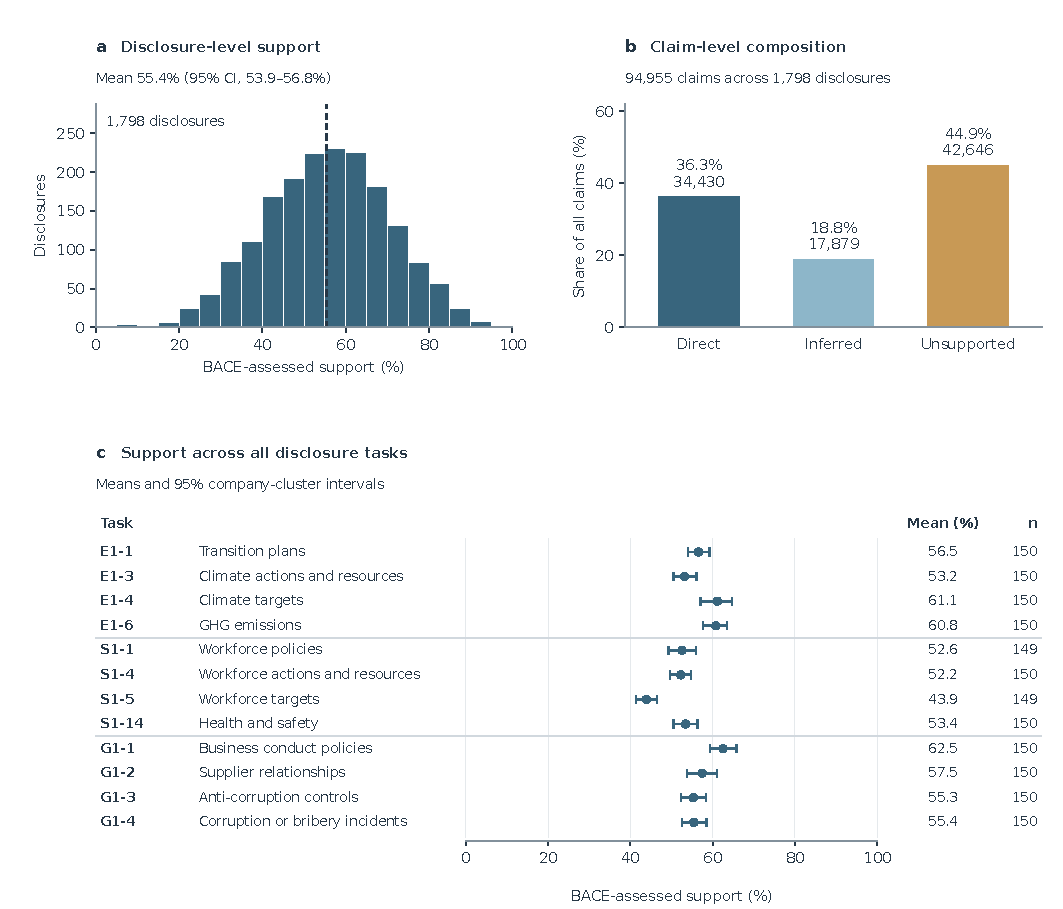
\includegraphics[width=\linewidth]{fig2_support.pdf}
\caption{\textbf{Evidentiary support across disclosure tasks.}
\textbf{a,} Distribution of BACE-assessed support across 1,798 completed disclosures from 30 companies, using 5-percentage-point bins.
Each disclosure's score is its number of directly or inferentially supported disclosure claims (DCs) divided by all its deduplicated DCs.
The dashed line marks the equally weighted disclosure mean of 55.4\% (95\% confidence interval, 53.9--56.8\%).
\textbf{b,} Pooled composition of all 94,955 DCs; labels give category percentages and counts.
Direct and inferred support together comprise 52,309 DCs (55.1\%).
This panel weights claims equally, whereas panels a and c weight disclosures equally.
All denominators retain non-disclosure statements.
\textbf{c,} Means and horizontal 95\% confidence intervals for all 12 tasks in protocol order, with abbreviated task topics.
The n column gives completed disclosures: 149 for S1-1 and S1-5 and 150 for each remaining task; every task includes 30 companies.
Intervals in a and c are the saved percentile company-cluster bootstrap intervals from 2,000 resamples, retaining all disclosures within each sampled company.
Two incomplete assessments are excluded without zero imputation.
Task variation is descriptive; no hypothesis test is reported.
BACE verdicts are conditional on the supplied evidence, extracted claims and selected candidate evidence.
These intervals describe company-resampling uncertainty, not the validity or model-run variability of those verdicts.}
\label{fig:2}
\end{figure}

\clearpage
\begin{figure}[!htbp]
\centering
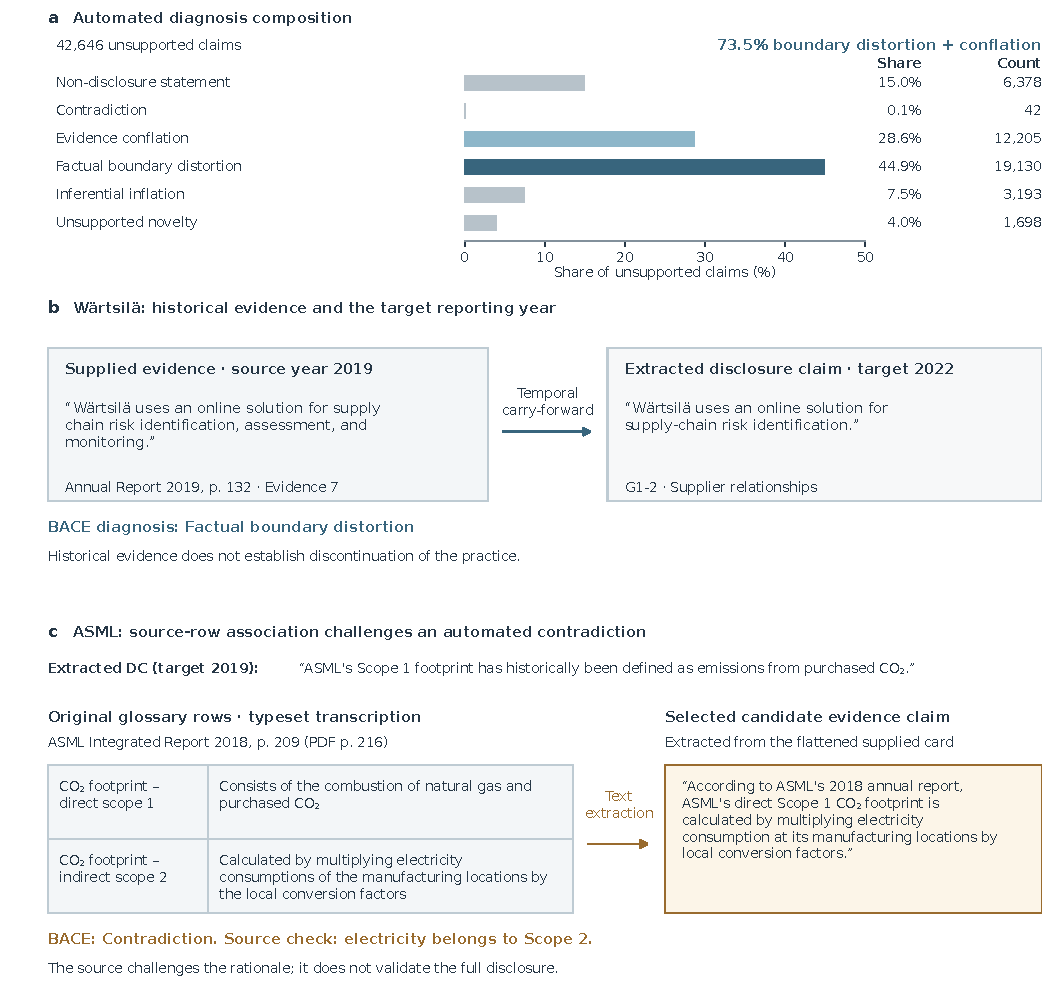
\includegraphics[width=\linewidth]{fig3_diagnoses_cases.pdf}
\caption{\textbf{Automated diagnoses and source-linked cases.}
\textbf{a,} Counts and percentages of the 42,646 unsupported disclosure claims (DCs) across 1,798 completed disclosures.
All six categories are retained in diagnostic-rule order, including non-disclosure statements.
Each unsupported DC receives one mutually exclusive label.
Factual boundary distortion and evidence conflation together account for 31,335 diagnoses (73.5\%).
These are descriptive pooled counts, with no confidence intervals or hypothesis tests; they do not estimate independently confirmed error prevalence.
\textbf{b,} The fixed Wärtsilä 2022 supplier-relationships example pairs a supplied excerpt from its 2019 Annual Report (p. 132) with the extracted DC.
BACE assigned factual boundary distortion; its rationale questions whether the historical description establishes target-year use.
The excerpt does not show that the practice ceased.
\textbf{c,} For the fixed ASML 2019 emissions example, two rows transcribed from the original Integrated Report 2018 glossary (printed p. 209; PDF p. 216) are juxtaposed with a selected candidate evidence claim.
Electricity conversion factors belong to indirect Scope 2 in the original layout but are associated with direct Scope 1 in the extracted claim.
This challenges the recorded contradiction rationale without validating the full disclosure.
The original page was inspected separately from the supplied flattened card.
Case excerpts are illustrative; complete selected-case evidence is retained in the source records.
Neither case constitutes representative or independent human validation.}
\label{fig:3}
\end{figure}

\clearpage
\begin{figure}[!htbp]
\centering
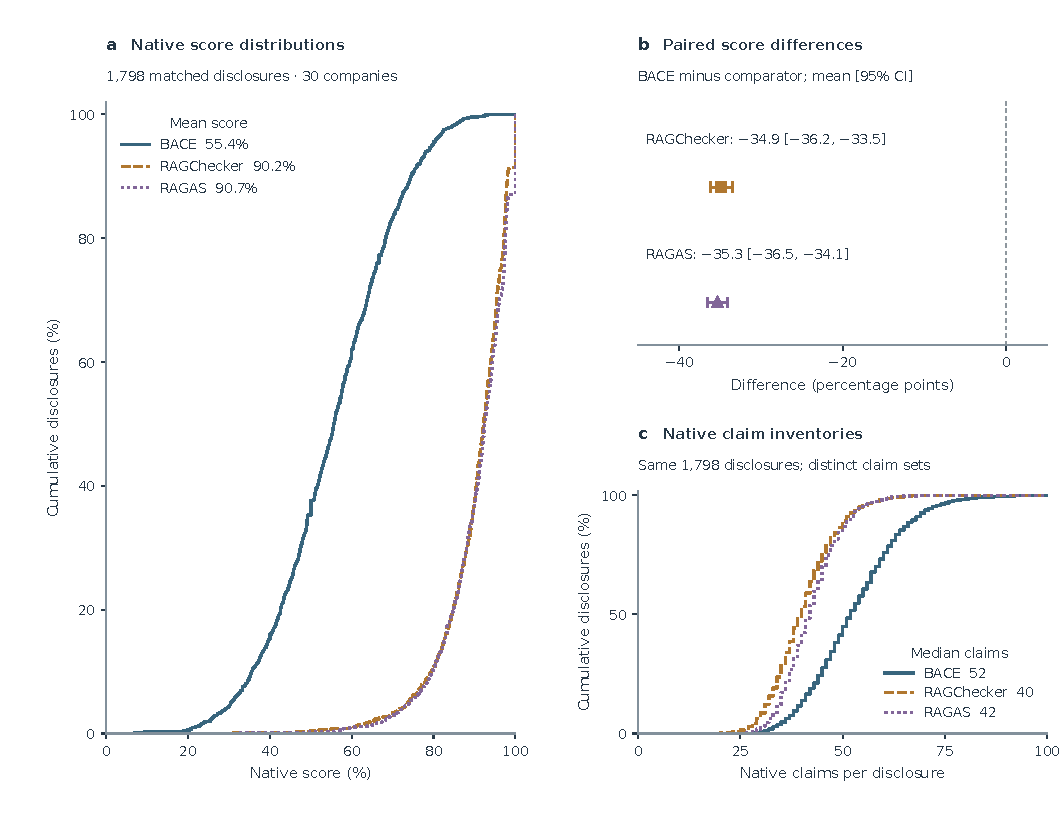
\includegraphics[width=\linewidth]{fig4_native_comparison.pdf}
\caption{\textbf{Native evaluator scores and claim inventories.}
All panels use the same 1,798 completed disclosures from 30 companies.
Two incomplete BACE assessments are excluded throughout without zero imputation.
\textbf{a,} Empirical cumulative distributions of native scores; each step gives the percentage of disclosures at or below the displayed value.
Legends report arithmetic mean scores.
BACE uses its all-disclosure-claim support rate, including non-disclosure statements; RAGChecker and RAGAS retain their native faithfulness scores.
\textbf{b,} Mean within-disclosure score differences, calculated as BACE minus each comparator, in percentage points.
Squares identify RAGChecker and triangles RAGAS.
Horizontal bars show saved 95\% percentile company-cluster bootstrap intervals from 2,000 resamples, retaining all disclosures within each sampled company.
Labels give means and interval limits; the dashed line marks zero difference.
No hypothesis test is reported.
\textbf{c,} Empirical cumulative distributions of native claim counts on the identical cohort, with medians in the legend.
The cumulative percentage refers to disclosures, not claims.
Both distributions retain every observation and count ties exactly, without smoothing or subsampling.
Pairing disclosures does not align the methods' claim inventories or judgment procedures.
Score gaps and inventory sizes do not establish comparative accuracy or a causal explanation for the gaps.
The intervals capture company-resampling uncertainty, not model-run variability or judgment validity.}
\label{fig:4}
\end{figure}

\clearpage
\end{document}
